% !Mode:: "TeX:UTF-8"
\chapter{实验设计}

我们针对本次研究设计了两个先导实验和两个用户实验。先导实验部分的主要目的是进行眼动确认信号的筛选和眼动操纵视线驻留检测优化方法的必要性探究;用户实验部分则是为了测试该对象操纵方法在单物体位移对接实验和多物体操纵“积木”实验中的效果。在实验过程中,我们会合理采集参试者的个人及实验数据,进行统计分析,并且从多客观度量和多主观度量对该对象操纵方法进行评估。我们的所有实验都基于表\ref{env}的环境条件:

% Please add the following required packages to your document preamble:
% \usepackage{multirow}
\begin{table}
\centering
\caption{实验环境条件}
\label{env}
\begin{tabular}{ccc}
\toprule
\textbf{类别}             & \textbf{项目}             & \textbf{规格}                      \\
\midrule
\multirow{2}{*}{VR硬件设备} & 头戴式显示器                  & Vive Focus 3                     \\
                        & 眼动追踪设备                  & Vive Focus 3 Eye Tracker         \\                
\midrule
\multirow{4}{*}{PC配置}   & 操作系统                    & Windows 11                       \\
                        & GPU                     & NVIDIA GeForce GTX 3060          \\
                        & CPU                     & 3.6GHz Intel(R)Core(TM)i7-9900KF \\
                        & RAM                     & 16GB                             \\
\midrule
\multirow{3}{*}{软件版本}   & Unity编辑器版本              & 2021.3.16f1                      \\
                        & Vive Business Streaming & 1.10.11                          \\
                        & SteamVR                 & 1.24.7                           \\
\midrule
参试者                     & 姿态                      & 固定坐姿                            \\
\bottomrule
\end{tabular}
\end{table}

\section{先导实验}

\subsection{实验1:眼动确认信号筛选}
\label{pilot-study-1}

\subsubsection{实验设计与流程}
此先导实验的目的是从最为常见且自然的两种主动眼动信号(单眼眨眼和快速两次眨眼)中确定一个最为高效并且带来最小使用压力的眼动确认信号。

我们招募了6名参试者;为了保证多样性,我们尽可能保证男女比例相当。参试者在开始实验前需填写一个个人信息调查问卷,以询问性别、工作机构、年龄和能否自然地完成单眼眨眼的动作等。我们的此次实验组由3名男性和3名女性构成,其中有3人无法自然地完成单眼眨眼的动作。

每名参试者将使用不同的两个眼动确认信号分两次完成同样的一个任务。该任务内容是,在虚拟环境中会依次在随机时刻和随机位置出现20个小球,参试者需要使用当次实验规定的眼动信号(单眼眨眼或快速两次眨眼)选择以消灭它们。为了保证每次实验结果的可比较性,我们规定:每个小球只有在参与者瞄准并且发出确认信号后才能消灭;下一个小球只有在当前小球被消灭后才生成;在每次发出确认信号前,参与者必须按下一次键盘上的空格键,以记录实际的信号尝试次数。

在实验完成后,每名参试者将分别针对两种确认信号完成一个NASA-TLX任务负担表。

\begin{table}[b!]
\centering
\caption{先导实验1:眼动确认信号筛选 - 实验结果}
\begin{tabular}{ccccccc}
\toprule
\multirow{2}{*}{\textbf{参试者}} & \multicolumn{3}{c}{\textbf{单眼眨眼}} & \multicolumn{3}{c}{\textbf{快速两次眨眼}} \\
  & 完成时间(ms) & NASA-TLX & FAI  & 完成时间(ms) & NASA-TLX & FAI  \\
\midrule
1(N) & 187621   & 92       & 0.43 & 105832   & 71       & 0.79 \\
2(Y) & 80122    & 71       & 0.87 & 113475   & 68       & 0.88 \\
3(N) & 161298   & 83       & 0.39 & 92103    & 79       & 0.91 \\
4(Y) & 89172    & 62       & 0.91 & 125764   & 73       & 0.76 \\
5(Y) & 90817    & 77       & 0.81 & 109675   & 91       & 0.86 \\
6(N) & 80012    & 89       & 0.49 & 98122    & 80       & 0.83 \\
\bottomrule
\end{tabular}
\label{table-4-1}
\end{table}

\subsubsection{实验度量}

我们将针对以下三个客观度量评估实验结果:

\begin{itemize}[wide]
	\item 任务完成时间(毫秒);
	\item 任务负担(NASA-TLX分数);
	\item 信号反馈精确系数(Feedback Accuracy Index, FAI)。我们规定在一次实验中,参试者实际消灭的小球数量为 $N$ ,总共发出的信号尝试次数为 $M$;则有FAI的计算规则:
	\begin{equation}
	FAI = \frac{N}{M}
	\label{formula-4-1}
	\end{equation}
\end{itemize}

本次先导实验的实验结果汇报见表\ref{table-4-1};其中,参试者编号后会标注该参试者能否自然地完成单眼眨眼动作(“Y”代表能,“N”代表否)。

我们采用曼-惠特尼U检验(Mann-Whitney U Test)来分析数据的显著差异性;该检验假设两个样本分别来自除了总体均值意外完全相同的两个总体,目的是检验这两个总体的均值是否有显著的差异。对于任务完成时间,检验结果是 $U = 18,\ p < 0.05$ ;对于任务负担,检验结果是 $U = 42,\ p < 0.05$ ;对于FAI,检验结果是 $U = 15.5,\ p < 0.05$ 。可以发现,三组结果皆存在显著差异;而快速两次眨眼均值表现更为理想,故可以确定快速两次眨眼显著优于单眼眨眼。

\subsection{实验2:眼动操纵视线驻留检测优化}

\subsubsection{实验设计与流程}

此先导实验的目的是是否有必要引入眼动操纵注视停留检测的优化。

此次实验的实验组和先导实验1(详见\ref{pilot-study-1})一致。每名参试者将分两次完成同样的一个任务;在两次的实验中,我们会随机在某一次引入优化以消除主观的心理作用干扰。该任务内容和先导实验1一致;我们规定在此次先导实验中,两次任务都使用快速两次眨眼作为确认信号。

\begin{table}[b!]
\centering
\caption{先导实验2:眼动操纵视线驻留检测优化 - 实验结果}
\begin{tabular}{cccc}
\toprule
\multirow{2}{*}{\textbf{参试者}} & \multirow{2}{*}{\textbf{\begin{tabular}[c]{@{}c@{}}引入优化组别\\ (参试者不可见)\end{tabular}}} & \textbf{含优化} & \textbf{不含优化} \\
  &   & NASA-TLX & NASA-TLX \\
\midrule
1 & 1 & 73       & 80       \\
2 & 2 & 47       & 53       \\
3 & 1 & 68       & 62       \\
4 & 2 & 75       & 83       \\
5 & 2 & 70       & 79       \\
6 & 1 & 82       & 86       \\
\bottomrule
\end{tabular}
\label{table-4-2}
\end{table}

在实验完成后,每名参试者将分别针对两次任务完成一个NASA-TLX任务负担表;由于用户在实验过程中并不知情某次任务是否引入优化,所以我们可以认为结果是客观的。

\subsubsection{实验度量}

我们将针对任务负担评估实验结果。

本次先导实验的实验结果汇报见表\ref{table-4-2}。

我们同样采用曼-惠特尼U检验来分析数据的显著差异性。对于任务负担,检验结果是 $U = 32,\ p < 0.05$ 。可以发现,两组结果存在显著差异,且引入优化组别和NASA-TLX结果不存在明显的相关性;而引入优化的任务负担均值表现更为理想,故此可以确定引入优化是必要的。

\section{用户实验}

为了消除偶然性、保证多样性,我们招募了14名参试者,并且尽可能确保男女比例相当。参试者在开始实验前需填写一个个人信息调查问卷,以询问性别、年龄、VR使用经验等。问卷结果显示,实验的受试组由8名男性和6名女性组成,年龄分布在20到38岁;其中有4人未曾有过VR使用经验,6人曾接触过VR使用,4人对VR使用非常熟悉。

\subsection{实验1:单物体位移对接实验}

\begin{figure}[b!]
    \centering
    \subfigure[位移空间]{
        \label{fig-4-1-l}
        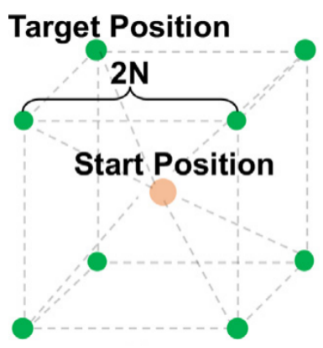
\includegraphics[width=.24\textwidth]{figure/user-study-1.png}
    }
    \hspace{5em} % 水平间隔
    \subfigure[场景实例]{
        \label{fig-4-1-r}
        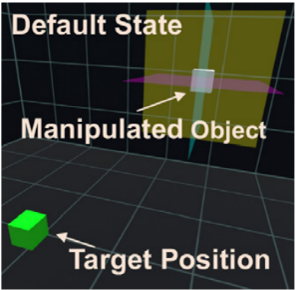
\includegraphics[width=.24\textwidth]{figure/user-study-2.png}
    }
    \caption{用户实验1:单物体位移对接实验}
    \label{fig-4-1}
\end{figure}

\subsubsection{实验设计}

我们将目前同样基于头眼协同的最优方法OrthoGaze中作为一个对照方法(CC)和基准线(baseline),并且复用其中的一个物体位移用户实验\upcite{2020Chang}。该用户实验设计为:参试者位于起始位置 $(0, 1[m], 0)$ 处,并尝试将大小为 $0.5[m] \times 0.5[m] \times 0.5[m]$ 的白色立方体从固定的起始位置 $\left(-1\ \left[m\right],\ 0.5\ \left[m\right],\ 5.5\ \left[m\right]\right)$ 移动到多个目标位置,如图\ref{fig-4-1-l}所示。在每次实验中,在目标位置上将出现一个半透明的、与白色立方体大小相同的绿色立方体;参试者必须将白色立方体与绿色立方体对齐,如图\ref{fig-4-1-r}所示。目标位置总是位于一个具有 $2N\left[m\right]$ 边长的立方体空间的角落,其中心与白色立方体的初始位置中心重合。我们使用了8个不同大小的立方体空间,其中 $N \in \left\{0.5,\ 1,\ 1.5,\ 2,\ 2.5,\ 3,\ 3.5,\ 4\right\}$ 。为了保持立方体对接的数量合理,该立方体空间的每个偏移方向都将被选择两次,并与每次出现的不同距离配对,从而确保每个偏移距离和方向在实验期间出现两次;这样,实验期间总共产生16个不同的目标位置。由于完全对齐白色和绿色立方体很困难,所以如果在用户确认放置时两个立方体之间距离小于阈值距离 $0.2\left[m\right]$ ,则认为对接成功。作为额外提示,当两个立方体在阈值距离内时,我们将目标立方体从半透明绿色变为红色。为了在一个试验中成功,参试者不仅需要将立方体移动到目标位置,还需要确认放置立方体。如果试验成功,参试者将收到一个声音反馈来确认。

\subsubsection{实验流程}

在开始实验之前,参试者将进行10次对接以练习该交互方法。在正式实验开始后,每一组任务从白色立方体和目标位置出现在参与者面前开始,并在对接成功后结束;如果参试者在20秒内没有对齐立方体,则本次任务将被视为失败。

在全部任务完成后,用户需要完成3个主观调查问卷:SSQ(Simulator Sickness Questionnaire)晕动症状问卷、SUS(System Usability Scale)可用性调查问卷和NASA-TLX(NASA Task Load Index)任务负荷问卷。

\begin{table}[]
\centering
\caption{用户实验1:单物体位移对接实验 - 实验结果}
\scalebox{0.9}{
\begin{tabular}{cccccccccccc}
\toprule
\multirow{2}{*}{\textbf{参试者}} & \multirow{2}{*}{\textbf{\begin{tabular}[c]{@{}c@{}}VR\\ 经验\end{tabular}}} & \multicolumn{5}{c}{\textbf{我们的方法(EC)}}  & \multicolumn{5}{c}{\textbf{OrthoGaze(CC)}} \\
                              &                                  & 成功 & 完成时间$_1$ & SSQ$_3$ & SUS$_5$ & TLX$_7$ & 成功  & 完成时间$_2$ & SSQ$_4$  & SUS$_6$ & TLX$_8$ \\
\midrule
1  & 用过   & Y & 8.72s  & 28 & 87 & 28 & Y & 11.32s & 37 & 75 & 45 \\
2  & 熟练   & Y & 8.11s  & 31 & 85 & 18 & Y & 13.19s & 28 & 79 & 34 \\
3  & 用过   & Y & 9.19s  & 21 & 92 & 27 & Y & 14.94s & 31 & 81 & 27 \\
4  & 无 & Y & 9.50s   & 39 & 82 & 19 & Y & 10.09s & 39 & 68 & 49 \\
5  & 熟练   & Y & 8.44s  & 13 & 89 & 20 & Y & 13.56s & 21 & 78 & 31 \\
6  & 无 & Y & 8.98s  & 24 & 89 & 30 & Y & 12.34s & 30 & 86 & 38 \\
7  & 无 & Y & 11.51s & 29 & 90 & 29 & Y & 13.17s & 40 & 64 & 42 \\
8  & 熟练   & Y & 8.99s  & 18 & 93 & 23 & Y & 11.31s & 20 & 82 & 52 \\
9  & 用过   & Y & 9.08s  & 19 & 88 & 25 & Y & 12.44s & 33 & 83 & 30 \\
10 & 用过   & Y & 10.27s & 22 & 82 & 21 & Y & 13.58s & 32 & 81 & 26 \\
11 & 无 & Y & 8.33s  & 27 & 79 & 15 & Y & 11.72s & 39 & 76 & 48 \\
12 & 熟练   & Y & 9.01s  & 17 & 95 & 24 & Y & 9.86s  & 24 & 80 & 51 \\
13 & 用过   & Y & 10.25s & 29 & 71 & 31 & Y & 11.02s & 35 & 66 & 39 \\
14 & 用过   & Y & 12.29s & 11 & 96 & 19 & Y & 14.13s & 22 & 84 & 36 \\
\bottomrule
\end{tabular}
}
\label{table-4-3}
\end{table}

\subsubsection{实验度量}

我们将从三个主观度量和三个客观度量来评估每一个参试者的实验结果。主观度量:眩晕感(SSQ)、可用性(SUS)、任务负担(NASA-TLX)。

\begin{itemize}[wide]
	\item {\bf 成功率}:成功率是针对每个参与者计算的,是成功任务的次数与所有任务次数的比率。这评估了操作物体的总体效率,因为要成功完成一个任务需要全面考虑准确性和速度。若一次实验成功,则在表格的“成功”栏记录“Y”,否则记录“N”。
	\item {\bf 完成时间}:在每个成功完成的任务中,完成时间将被记录;对于此项度量,我们不会将失败的任务纳入考虑。我们会记录两组实验数据:包括和不包括凝视停留的时间。
	\item {\bf 最终距离}:此项度量仅针对失败的任务。最终距离是指在任务失败时刻白色立方体到目标位置的欧几里得距离(Euclidean Metric);我们将其归一化为最终距离除以初始距离。这种归一化反映了参试者在将物体移动到目标位置时相对于其初始位置的靠近/远离程度。
\end{itemize}

本次用户实验的实验结果汇报见表\ref{table-4-3}。由于全部实验都成功,所以我们不再考量最终距离指标。

\begin{figure}[b!]
    \centering
    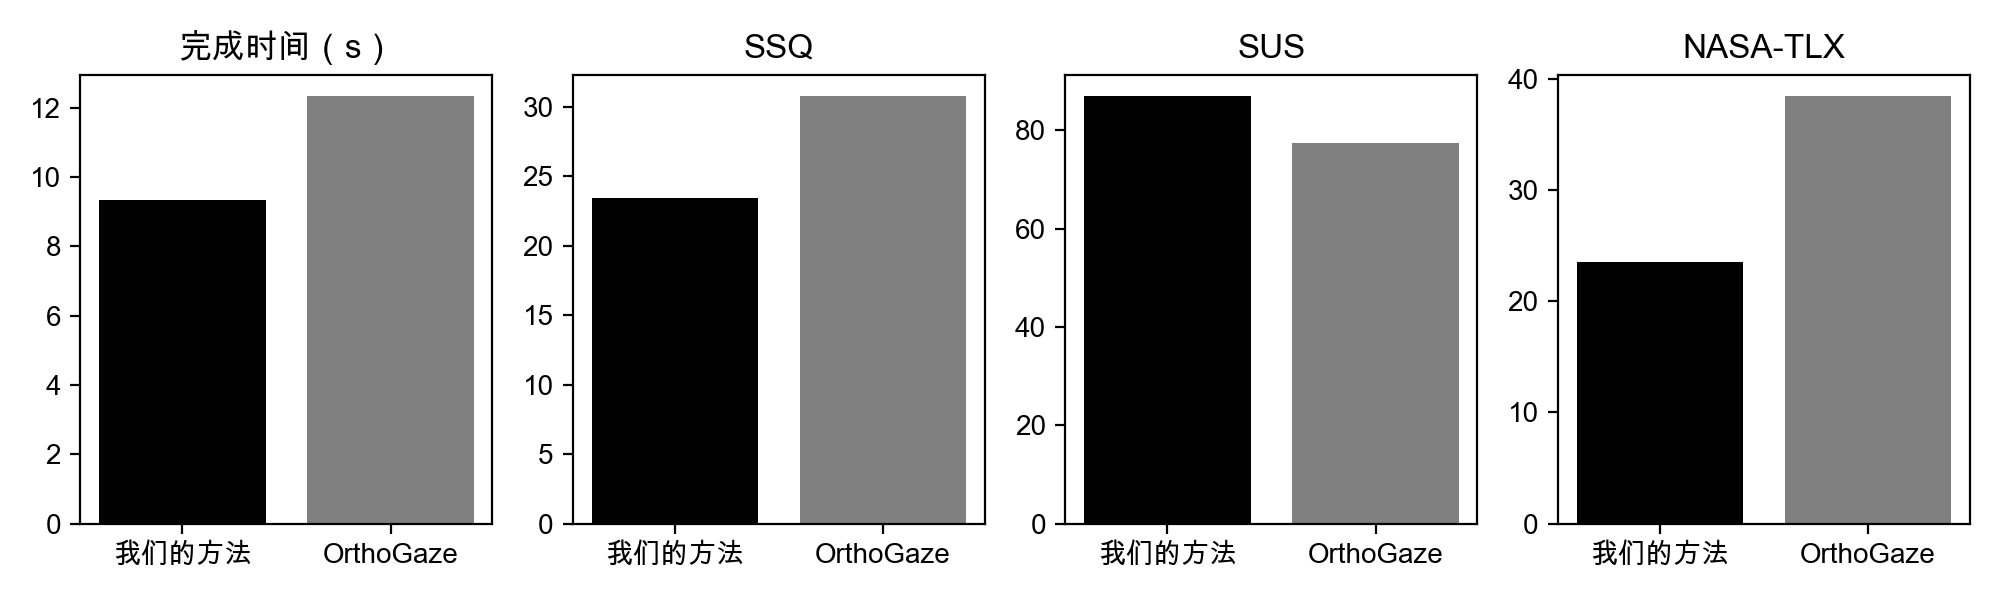
\includegraphics[width=\textwidth]{figure/user-study-1-avg.png}
    \caption{用户实验1:单物体位移对接实验 - 均值对比}
    \label{fig-4-2}
\end{figure}

本次实验的均值比较情况见图\ref{fig-4-2},可以清晰地观察到EC的效果是全面优于CC的。在本次实验中含一个自变量(因子)和一个因变量(响应变量):自变量为操纵方法,是一个分类变量;因变量为完成时间等结果数据,是一个连续变量。同时,所有样本都是独立的,并且通过Shapiro-Wilk检验发现数据皆呈正态分布( $p_1 = 0.192 > 0.05, p_2 = 0.886 > 0.05, p_3 = 0.958 > 0.05, p_4 = 0.284 > 0.05, p_5 = 0.443 > 0.05, p_6 = 0.083 > 0.05, p_7 = 0.671 > 0.05, p_8 = 0.821 > 0.05$ )。另外,Levene检验表明比较数据间方差齐性假设成立( $p_{12} = 0.061 > 0.05, p_{34} = 0.745 > 0.05, p_{56} = 0.969 > 0.05, p_{78} = 0.076 > 0.05$ )。所以,我们可以通过一元方差分析(One-Way ANOVA)来获取两种对比方法的差异显著性;检验表明,
EC与CC在完成时间( $F_{12}[1, 26] = 39.445, p_{12} = 1.20 \times 10^{-6} < 0.05$ )、
SSQ( $F_{34}[1, 26] = 7.119, p_{34} = 0.0130 < 0.05$ )、
SUS( $F_{56}[1, 26] = 13.995, p_{56} = 0.000915 < 0.05$ )、
NASA-TLX( $F_{78}[1, 26] = 33.440, p_{78} = 4.32 \times 10^{-6} < 0.05$ )上皆有显著差异。故此,我们可以得出结论:我们的方法在使用效率和用户体验上显著优于同类最优方法OrthoGaze。

同时,我们可以通过分析由我们的方法产出的实验结果是否会因为参试者的VR经验不同而导致显著差异来判断我们的方法是否易于学习。所以,我们提取出三种VR使用经验(无、用过、熟练)分别对应的完成时间数据到表\ref{table-4-4}。根据一元方差分析,三种VR经验对应的完成时间数据没有显著差异( $F[2, 11] = 2.31, p = 0.1477 > 0.05$ )。故此,我们也可以得出结论:我们的方法具备高可学习性。

\begin{table}[t!]
\centering
\caption{用户实验1:单物体位移对接实验 - VR经验对应完成时间}
\begin{tabular}{ccccccc}
\toprule
\textbf{VR使用经验} & \multicolumn{6}{c}{\textbf{完成时间}} \\
\midrule
无 & 9.50 & 8.98 & 11.51 & 8.33  &       &       \\
用过   & 8.72 & 9.19 & 9.08  & 10.27 & 10.25 & 12.29 \\
熟练   & 8.11 & 8.44 & 8.99  & 9.01  &       &       \\
\bottomrule
\end{tabular}
\label{table-4-4}
\end{table}

\subsection{实验2:多物体操纵“积木”实验}

\subsubsection{实验设计}

用户实验2延续用户实验1的受试组。

\begin{figure}[b!]
    \centering
    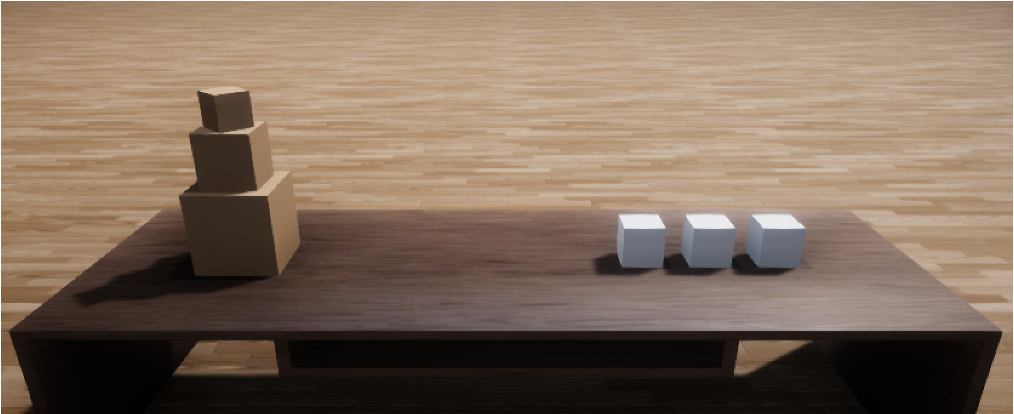
\includegraphics[width=0.75\textwidth]{figure/user-study-2-screenshot.png}
    \caption{用户实验2:多物体操纵“积木”实验 - 虚拟场景}
    \label{fig-4-3}
\end{figure}

在这个实验中,参试者将被要求分别使用我们的基于头眼协同的方法和两个对照方法完成一个“积木”实验。在一次“积木”实验中,我们确保必要操纵动作包含位移、缩放和旋转。在实验的虚拟场景中固定放置有一张长桌;桌面左侧是随机生成的不带碰撞检测的刚体棕色目标积木形状,右侧是用户可操纵的带碰撞检测的刚体白色积木块;可操纵的积木块数固定为3,且形状全为立方体,因为立方体放置稳固且可以直观体现缩放和旋转的效果(见图\ref{fig-4-3})。在每次实验中,参试者需要尽快将右侧的积木通过位移、旋转、缩放搭建为左侧的目标形状。

\subsubsection{实验流程}

我们在本次实验中设置两个对照组;参试者将分别使用我们的方法(EC)、PRISM方法(CC$_1$)\upcite{2017Kim}和目前基于凝视和手的最优方法Implicit Gaze(CC$_2$)\upcite{2021Yu}完成3次独立实验,每次实验有60s的完成时间。同时,系统实时用豪斯多夫距离(Hausdorff Distance)计算与目标积木形状的相似度\upcite{hausdorff}。在实验完成时间内,一旦豪斯多夫距离小于某一阈值(在此我们设定为0.2),则认定实验成功,记录完成时间,本次试验结束;超出完成时间,则认定实验失败,实验结束,记录此时的豪斯多夫距离,作为最终距离。全部参试者完成实验后,我们计算实验成功率,统计完成时间(仅针对成功的实验),统计最终距离(仅针对失败的实验),并最终以这三个客观度量评估实验结果。

\subsubsection{实验度量}

本次用户实验的实验结果汇报见表\ref{table-4-5}。

\begin{figure}[t!]
    \centering
    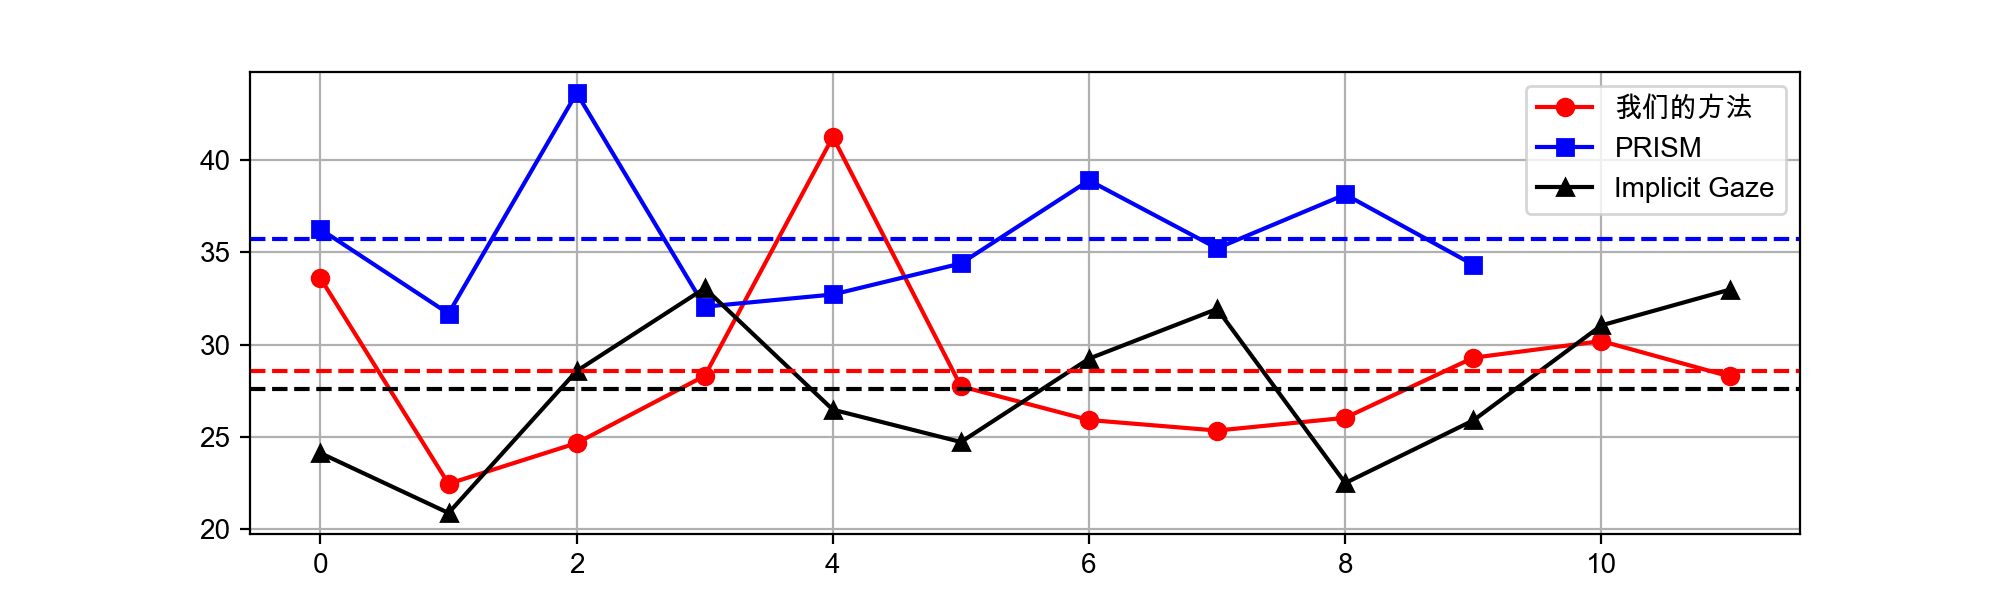
\includegraphics[width=\textwidth]{figure/user-study-2-avg.png}
    \caption{用户实验2:多物体操纵“积木”实验 - 均值对比}
    \label{fig-4-4}
\end{figure}

% Please add the following required packages to your document preamble:
% \usepackage{multirow}
\begin{table}[b!]
\centering
\caption{用户实验2:多物体操纵“积木”实验 - 实验结果}
\begin{tabular}{cccccccccc}
\toprule
\multirow{2}{*}{\textbf{参试者}} &
  \multicolumn{3}{c}{\textbf{我们的方法(EC)}} &
  \multicolumn{3}{c}{\textbf{PRISM(CC$_1$)}} &
  \multicolumn{3}{c}{\textbf{Implicit Gaze(CC$_2$)}} \\
 &
  成功 &
  \begin{tabular}[c]{@{}c@{}}完成\\ 时间$_1$\end{tabular} &
  \begin{tabular}[c]{@{}c@{}}最终\\ 距离$_4$\end{tabular} &
  成功 &
  \begin{tabular}[c]{@{}c@{}}完成\\ 时间$_2$\end{tabular} &
  \begin{tabular}[c]{@{}c@{}}最终\\ 距离$_5$\end{tabular} &
  成功 &
  \begin{tabular}[c]{@{}c@{}}完成\\ 时间$_3$\end{tabular} &
  \begin{tabular}[c]{@{}c@{}}最终\\ 距离$_6$\end{tabular} \\
\midrule
1  & Y & 33.59 &      & Y & 36.24 &      & Y & 24.13 &      \\
2  & N &       & 0.32 & N &       & 0.21 & Y & 20.89 &      \\
3  & Y & 22.47 &      & Y & 31.68 &      & Y & 28.57 &      \\
4  & Y & 24.67 &      & Y & 43.61 &      & Y & 33.05 &      \\
5  & Y & 28.31 &      & Y & 32.05 &      & N &       & 0.28 \\
6  & Y & 41.23 &      & Y & 32.71 &      & Y & 26.48 &      \\
7  & Y & 27.74 &      & N &       & 0.52 & Y & 24.73 &      \\
8  & Y & 25.92 &      & Y & 34.39 &      & Y & 29.24 &      \\
9  & Y & 25.35 &      & Y & 38.88 &      & Y & 31.93 &      \\
10 & N &       & 0.25 & N &       & 0.36 & Y & 22.51 &      \\
11 & Y & 26.04 &      & N &       & 0.47 & Y & 25.9  &      \\
12 & Y & 29.29 &      & Y & 35.21 &      & Y & 31.04 &      \\
13 & Y & 24.19 &      & Y & 38.12 &      & Y & 32.97 &      \\
14 & Y & 28.28 &      & Y & 34.32 &      & N &       & 0.29 \\
\bottomrule
\end{tabular}
\label{table-4-5}
\end{table}

三种方法产出的有效完成时间的均值情况见图\ref{fig-4-4},其中虚线即代表对应数据的均值。我们首先对三种对比方法产出的完成时间进行差异显著性分析。通过Shapiro-Wilk检验,我们发现三组完成时间都符合正态分布( $p_1 = 0.155 > 0.05, p_2 = 0.139 > 0.05, p_3 = 0.843 > 0.05$ );另外,Levene检验表明比较数据间方差齐性假设成立( $p_{123} = 0.788 > 0.05$ )。所以,我们可以使用一元方差分析来检验数据间的差异显著性;分析显示,三组之间至少有两组存在显著差异( $F_{123}[2, 31] = 7.119, p_{123} = 0.000219 < 0.05$ )。随后,我们进行Tukey HSD事后检验,发现差异来源主要为EC和CC$_1$以及CC$_2$和CC$_1$。根据均值表现,我们可以得出结论:我们的方法在操纵效率上显著优于PRISM,并且和Implicit Gaze无显著差异。随后,我们进行对成功率和最终距离的分析。EC的成功率为85.7\%,高于CC$_1$的71.4\%,并且和CC$_2$的成功率保持一致。在最终距离上,通过一元方差分析,三种方法的最终距离无显著差异( $F_{456}[2, 5] = 0.933, p_{456} = 0.453 > 0.05$ )。故此可以得出结论:虽然三种方法的最大尝试程度没有显著差异,但我们的方法和Implicit Gaze都优于PRISM,具有可观的成功率。

目前对象操纵方法中最优的即基于手的方法,而PRISM是变体最多、最广泛使用的基于手的方法之一,同时Implicit Gaze是基于手的对象操纵方法中的最优方法\upcite{2021Monteiro}。综上所述,我们可以得出结论:该头眼协同方法不亚于任何基于手的方法,并且在效率上显著优于PRISM方法。

